\documentclass[10pt,twocolumn,letterpaper]{article}

% CVPR 2026 author-kit style sheet (cvpr.sty, in this folder).  It already
% provides times, xcolor, graphicx, amsmath, amssymb, booktabs, natbib,
% caption and subcaption -- do not load those again, and do not load geometry,
% which would override the page layout cvpr.sty sets.
\usepackage{cvpr}

\definecolor{cvprblue}{rgb}{0.21,0.49,0.74}
\usepackage[pagebackref,breaklinks,colorlinks,allcolors=cvprblue]{hyperref}

\def\paperID{0000}
\def\confName{CVPR}
\def\confYear{2026}

% on a float-only page, stack floats from the top instead of spreading them
\makeatletter
\setlength{\@fptop}{0pt}
\makeatother

\title{\textbf{EECS 4422 Computer Vision}\\[4pt]
       \large Frequency-Domain Deblurring}
\author{Simon Posluns - 221541727 - simonp22@my.yorku.ca}
\date{}

\begin{document}

\maketitle

\section*{Implementing and comparing Fourier-domain restoration methods for deblurring}

\subsection*{Image source}

Clean reference images are taken from \textbf{CBSD68} (68 colour natural images,
$321 \times 481$), obtained from the benchmark collection at
\url{https://github.com/majedelhelou/denoising_datasets}.

\subsection*{Degradation model — Synthetically blurring the input images}

Following the course notation, $g$ denotes the original image and $f$ the degraded
observation:
\begin{align}
  f(x,y) &= h(x,y) * g(x,y) + n(x,y) \\
  F(u,v) &= H(u,v)\,G(u,v) + N(u,v)
\end{align}

\noindent $g$ = original (sharp) image, $h$ = blur kernel (PSF), $n$ = additive noise,
$f$ = observed blurry image; capitals denote the corresponding 2-D discrete Fourier
transforms, and $\hat{G}$ denotes the restored estimate of $G$.

\subsubsection*{What the blurring operation does}

Applies a convolution:
\begin{align}
  (h * g)(x,y) &= \sum_{i}\sum_{j} h(i,j)\, g(x-i,\; y-j)
\end{align}

\noindent The kernel used here is an isotropic Gaussian of width $\sigma$, normalised to unit sum:
\begin{align}
  h(x,y) &= \frac{1}{2\pi\sigma^{2}}
            \exp\!\left(-\frac{x^{2}+y^{2}}{2\sigma^{2}}\right),
  \qquad \sum_{x,y} h(x,y) = 1
\end{align}

\noindent Because the weights sum to one, the local average is preserved, so blurring
redistributes intensity without changing overall brightness. The kernel is evaluated on an
odd window of half-width $\lceil 3\sigma \rceil$, beyond which its values are negligible.

\noindent The filter is applied separately.

\newpage
\subsection*{Inverse filter}

By the convolution theorem, convolution in the spatial domain becomes multiplication in the
frequency domain:
\begin{align}
  g * h \quad&\Longleftrightarrow\quad G\,H
\end{align}

\noindent Applying this to the degradation model turns the convolution into a product:
\begin{align}
  f = h * g + n
  \quad&\Longleftrightarrow\quad
  F = H\,G + N
\end{align}

\noindent Considering the Fourier transforms of $g$, $f$ and $h$, (we assume $\text{noise} = 0$) :

\begin{align}
  G(u,v) &= \text{the sharp image to recover,} \\
  F(u,v) &= \text{the blurred image} \\
  H(u,v) &= \text{the blur, as a gain applied to each frequency.}
\end{align}

\noindent Blurring multiplies $G$ by $H$, so the restoration divides it back out:
\begin{align}
  \hat{G} &= \frac{F}{H}
\end{align}

\noindent Since $|H|$ becomes vanishingly small at high frequencies, it is floored at
$\varepsilon$ before dividing (to avoid division by 0):
\begin{align}
  \hat{G}(u,v) &= \frac{F(u,v)}{H_{\varepsilon}(u,v)},
  \qquad
  H_{\varepsilon} =
  \begin{cases}
    H,          & |H| \ge \varepsilon, \\
    \varepsilon, & |H| < \varepsilon,
  \end{cases}
  \qquad \varepsilon = 10^{-2}
\end{align}

\subsubsection*{Steps}

\begin{enumerate}
  \item Build the kernel $h$ from $\sigma$, then transform it: $H = \mathcal{F}\{h\}$.
        A Gaussian is fully determined by $\sigma$, so no other information is needed, and
        this is the identical $H$ that produced the blur.
  \item Floor it: $H_{\varepsilon} = \max(|H|,\ \varepsilon)$, keeping $H$ elsewhere.
  \item For each colour channel:
    \begin{enumerate}
      \item $F = \mathcal{F}\{f\}$ \hfill (pixels $\to$ frequencies)
      \item $\hat{G} = F / H_{\varepsilon}$ \hfill (divide out the blur)
      \item $\hat{g} = \operatorname{Re}\,\mathcal{F}^{-1}\{\hat{G}\}$
            \hfill (frequencies $\to$ pixels)
       \item keep the real part of output, discard the imaginary part,
    \end{enumerate}
\end{enumerate}

\newpage
\subsection*{Wiener filter}

Rather than assume $n = 0$, find the linear shift-invariant filter $w$ minimising the expected
mean square error between the estimate $\hat{g} = w * f$ and the original image $g$:
\begin{align}
  \min_{w} \; \mathbb{E}\!\left[\,\iint \bigl(\hat{g}(x,y) - g(x,y)\bigr)^{2} dx\,dy\,\right]
\end{align}

\noindent The solution is expressed in terms of \emph{power spectral densities} (PSDs)
--- the expected energy each signal carries at each frequency --- of the original image,
the noise, and the degraded image respectively:
\begin{align}
  P_{g}(u,v) &= \mathbb{E}\!\left[\left|G(u,v)\right|^{2}\right] \\
  P_{n}(u,v) &= \mathbb{E}\!\left[\left|N(u,v)\right|^{2}\right] \\
  P_{f}(u,v) &= \mathbb{E}\!\left[\left|F(u,v)\right|^{2}\right]
\end{align}

\noindent Substituting $F = H G + N$ into $P_{f} = \mathbb{E}\!\left[|F|^{2}\right]$ and
expanding with $\left|a + b\right|^{2} = \left|a\right|^{2} + \left|b\right|^{2}
+ 2\operatorname{Re}\left(a b^{*}\right)$:
\begin{align}
  P_{f} &= \mathbb{E}\!\left[\left|H G + N\right|^{2}\right] \nonumber \\
        &= \left|H\right|^{2}\mathbb{E}\!\left[\left|G\right|^{2}\right]
           + \mathbb{E}\!\left[\left|N\right|^{2}\right]
           + 2\operatorname{Re}\mathbb{E}\!\left[H G N^{*}\right]
\end{align}

\noindent The cross term vanishes because $H$ is deterministic, $G$ and $N$ are independent,
and the noise has zero mean:
\begin{align}
  \mathbb{E}\!\left[H G N^{*}\right]
    &= H\,\mathbb{E}\!\left[G N^{*}\right]
     = H\,\mathbb{E}\!\left[G\right]\mathbb{E}\!\left[N^{*}\right]
     = 0
\end{align}

\noindent Thus:
\begin{align}
  P_{f} &= \left|H\right|^{2} P_{g} + P_{n}
\end{align}

\noindent The best $W$ is the one that leaves an error independent of the data: if the error
still depended on the data, adjusting $W$ could remove more of it.
\begin{align}
  \mathbb{E}\!\left[\left(W F - G\right) F^{*}\right] &= 0
\end{align}

\noindent Rearranging, then substituting $F = H G + N$ and dropping the cross term as before:
\begin{align}
  W &= \frac{\mathbb{E}\!\left[G F^{*}\right]}{\mathbb{E}\!\left[\left|F\right|^{2}\right]}
     = \frac{H^{*} P_{g}}{P_{f}}
     = \frac{H^{*} P_{g}}{\left|H\right|^{2} P_{g} + P_{n}}
\end{align}

\noindent That is, $W \approx 1/H$ where the signal dominates and $W \approx 0$ where the
noise does. Writing $K = P_{n}/P_{g}$:
\begin{align}
  \hat{G}(u,v) &= \frac{H^{*}(u,v)}{\left|H(u,v)\right|^{2} + K}\;F(u,v),
  \qquad K = 3 \times 10^{-4}
\end{align}

\noindent The denominator cannot reach zero, so no $\varepsilon$-floor is needed;
$K \to 0$ recovers the inverse filter.

\subsubsection*{Steps}

\begin{enumerate}
  \item Build the kernel $h$ from $\sigma$, then transform it: $H = \mathcal{F}\{h\}$.
  \item Form the filter once: $W = H^{*} / \left(\left|H\right|^{2} + K\right)$.
  \item For each colour channel:
    \begin{enumerate}
      \item $F = \mathcal{F}\{f\}$ \hfill (pixels $\to$ frequencies)
      \item $\hat{G} = W\,F$ \hfill (apply the filter)
      \item $\hat{g} = \operatorname{Re}\,\mathcal{F}^{-1}\{\hat{G}\}$
            \hfill (frequencies $\to$ pixels)
    \end{enumerate}
\end{enumerate}

\noindent \emph{Note:} both the estimation of $K = P_{n}/P_{g}$ and the actual oracle values
from original image are used in comparison in the functions \texttt{wiener\_filter} and
\texttt{wiener\_filter\_oracle}.


\newpage
\subsection*{Constrained least squares (Laplacian)}

The Wiener filter needs $P_{n}$ and $P_{g}$, which are unknown in general. Constrained least
squares replaces those statistics with a preference: among all estimates consistent with the
data, choose the smoothest. Roughness is measured by the Laplacian, $\nabla^{2}$, the sum of
the second derivative along each axis:
\begin{align}
  \nabla^{2} g &= \frac{\partial^{2} g}{\partial x^{2}}
                + \frac{\partial^{2} g}{\partial y^{2}}
\end{align}

\noindent Differencing twice along $x$ gives the discrete form of each term:
\begin{align}
  \frac{\partial^{2} g}{\partial x^{2}}
    &\approx \bigl[g(x{+}1) - g(x)\bigr] - \bigl[g(x) - g(x{-}1)\bigr] \nonumber \\
    &= g(x{+}1) - 2g(x) + g(x{-}1)
\end{align}

\noindent so each axis contributes the kernel $[\,1\ \ {-2}\ \ 1\,]$, and their sum is the
$3 \times 3$ operator $p$:
\begin{align}
  p &=
  \begin{bmatrix}
    0 & 0 & 0 \\
    1 & -2 & 1 \\
    0 & 0 & 0
  \end{bmatrix}
  +
  \begin{bmatrix}
    0 & 1 & 0 \\
    0 & -2 & 0 \\
    0 & 1 & 0
  \end{bmatrix}
  =
  \begin{bmatrix}
    0 &  1 & 0 \\
    1 & -4 & 1 \\
    0 &  1 & 0
  \end{bmatrix}
\end{align}

\noindent Its weights sum to zero, so a region of constant intensity gives exactly zero
response: the operator measures curvature only, and is blind to brightness.

\noindent Minimise that roughness subject to the estimate reproducing the observed image:
\begin{align}
  \min_{\hat{g}} \; \left\lVert p * \hat{g} \right\rVert^{2}
  \qquad \text{subject to} \qquad
  \left\lVert f - h * \hat{g} \right\rVert^{2} &= \left\lVert n \right\rVert^{2}
\end{align}

\noindent Introducing a multiplier $\gamma$ for the constraint and setting the derivative of
the combined objective to zero gives, in the frequency domain:
\begin{align}
  \hat{G}(u,v) &= \frac{H^{*}(u,v)}
                       {\left|H(u,v)\right|^{2} + \gamma\left|P(u,v)\right|^{2}}\;F(u,v),
  \qquad \gamma = 10^{-4}
\end{align}

\noindent where $P = \mathcal{F}\{p\}$. This is the Wiener filter with the constant $K$
replaced by $\gamma\left|P\right|^{2}$. Because $p$ is high-pass, that penalty varies with
frequency:
\begin{align}
  P(0,0) &= 0
    &&\text{the mean is unconstrained,} \\
  \left|P\right|^{2} &\to 64
    &&\text{maximal penalty at the highest frequencies.}
\end{align}

\noindent So the damping is applied exactly where the inverse filter fails, and no noise
statistics are required --- only the assumption that the original image is smooth.

\subsubsection*{Steps}

\begin{enumerate}
  \item Build the kernel $h$ from $\sigma$ and transform it: $H = \mathcal{F}\{h\}$.
  \item Build the Laplacian $p$ on the same grid and transform it: $P = \mathcal{F}\{p\}$.
  \item Form the filter once:
        $W = H^{*} / \left(\left|H\right|^{2} + \gamma\left|P\right|^{2}\right)$.
  \item For each colour channel:
    \begin{enumerate}
      \item $F = \mathcal{F}\{f\}$ \hfill (pixels $\to$ frequencies)
      \item $\hat{G} = W\,F$ \hfill (apply the filter)
      \item $\hat{g} = \operatorname{Re}\,\mathcal{F}^{-1}\{\hat{G}\}$
            \hfill (frequencies $\to$ pixels)
    \end{enumerate}
\end{enumerate}

\newpage
% LaTeX always defers a double-column float (table*/figure*) to a later page, so
% these are set as plain full-width content with \captionof instead -- that is
% what keeps the paragraph, the table and the chart together on one page.
\clearpage
\onecolumn

\subsection*{Results}

All four filters are run over the same 68 CBSD68 images, blurred with $\sigma = 2$ and
written to 8-bit PNG, so the only noise present is the quantisation of that round trip.
Each restored image is clipped to $[0,1]$ before scoring. PSNR measures squared error;
SSIM compares local mean, contrast and correlation over a $7 \times 7$ window, so the
two disagree where a method trades error for structure.

\vspace{1em}

\begin{center}
  \begin{tabular}{lrrrr}
\toprule
Method & PSNR (dB) & $\Delta$ PSNR & SSIM & ms/image \\
\midrule
Blurry input & 24.29 & --- & 0.6703 & --- \\
\midrule
Inverse filter & 19.50 & -4.79 & 0.3454 & 24 \\
Wiener filter & 27.84 & +3.56 & 0.8242 & 24 \\
Wiener filter (oracle) & 28.19 & +3.90 & 0.8259 & 36 \\
Constrained least squares & 27.84 & +3.55 & 0.8263 & 27 \\
\bottomrule
\end{tabular}

  \captionof{table}{Mean PSNR and SSIM over 68 images, $\sigma = 2$.}
\end{center}

\vspace{1em}

\begin{center}
  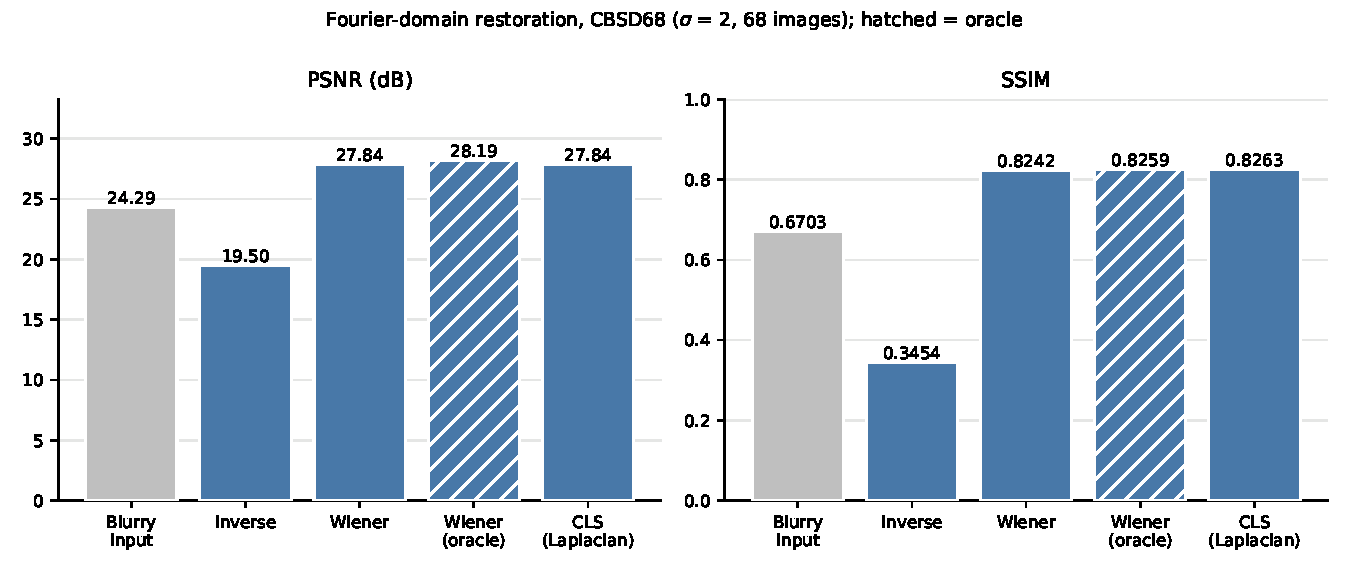
\includegraphics[width=0.78\linewidth]{results.pdf}
  \captionof{figure}{The same figures. The oracle (hatched) uses the ground-truth
  $P_{g}$, so it is an upper bound rather than an achievable result.}
\end{center}



\clearpage
\subsection*{Sample restorations}

\noindent One grid per image, each cell captioned with its own PSNR and SSIM against
the ground truth. Generated by \texttt{save\_panels()}, so the scores below cannot
drift from those in Table 1.

% one 3x2 portrait grid per sample image
\begin{center}
  \begin{minipage}{0.48\linewidth}\centering
    
\includegraphics[width=\linewidth]{../blurred/sigma_2/3096.png}\\[2pt]
    {\footnotesize Blurry input --- 32.95\,dB / 0.9526}
  \end{minipage}%
  \hfill
  \begin{minipage}{0.48\linewidth}\centering
    
\includegraphics[width=\linewidth]{../deblurred-imgs/inverse/3096.png}\\[2pt]
    {\footnotesize Inverse filter --- 19.99\,dB / 0.1362}
  \end{minipage}
  \\[8pt]
  \begin{minipage}{0.48\linewidth}\centering
    
\includegraphics[width=\linewidth]{../deblurred-imgs/wiener/3096.png}\\[2pt]
    {\footnotesize Wiener filter --- 36.01\,dB / 0.8970}
  \end{minipage}%
  \hfill
  \begin{minipage}{0.48\linewidth}\centering
    
\includegraphics[width=\linewidth]{../deblurred-imgs/wiener-oracle/3096.png}\\[2pt]
    {\footnotesize Wiener filter (oracle) --- 37.12\,dB / 0.9514}
  \end{minipage}
  \\[8pt]
  \begin{minipage}{0.48\linewidth}\centering
    
\includegraphics[width=\linewidth]{../deblurred-imgs/cls-laplacian/3096.png}\\[2pt]
    {\footnotesize Constrained least squares --- 36.22\,dB / 0.9073}
  \end{minipage}%
  \hfill
  \begin{minipage}{0.48\linewidth}\centering
    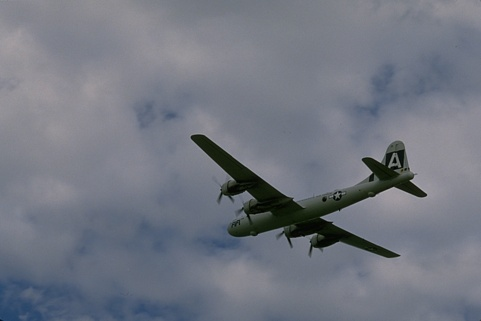
\includegraphics[width=\linewidth]{../../CBSD68/3096.png}\\[2pt]
    {\footnotesize Ground truth}
  \end{minipage}
  \\[8pt]
  \captionof{figure}{\texttt{3096.png} restored from $\sigma = 2$ blur. Read left to right, top to bottom.}
\end{center}

\clearpage
\begin{center}
  \begin{minipage}{0.48\linewidth}\centering
    
\includegraphics[width=\linewidth]{../blurred/sigma_2/12084.png}\\[2pt]
    {\footnotesize Blurry input --- 24.35\,dB / 0.6417}
  \end{minipage}%
  \hfill
  \begin{minipage}{0.48\linewidth}\centering
    
\includegraphics[width=\linewidth]{../deblurred-imgs/inverse/12084.png}\\[2pt]
    {\footnotesize Inverse filter --- 19.46\,dB / 0.4008}
  \end{minipage}
  \\[8pt]
  \begin{minipage}{0.48\linewidth}\centering
    
\includegraphics[width=\linewidth]{../deblurred-imgs/wiener/12084.png}\\[2pt]
    {\footnotesize Wiener filter --- 29.22\,dB / 0.8687}
  \end{minipage}%
  \hfill
  \begin{minipage}{0.48\linewidth}\centering
    
\includegraphics[width=\linewidth]{../deblurred-imgs/wiener-oracle/12084.png}\\[2pt]
    {\footnotesize Wiener filter (oracle) --- 29.48\,dB / 0.8699}
  \end{minipage}
  \\[8pt]
  \begin{minipage}{0.48\linewidth}\centering
    
\includegraphics[width=\linewidth]{../deblurred-imgs/cls-laplacian/12084.png}\\[2pt]
    {\footnotesize Constrained least squares --- 29.19\,dB / 0.8693}
  \end{minipage}%
  \hfill
  \begin{minipage}{0.48\linewidth}\centering
    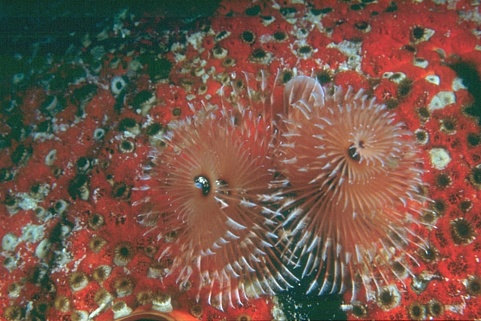
\includegraphics[width=\linewidth]{../../CBSD68/12084.png}\\[2pt]
    {\footnotesize Ground truth}
  \end{minipage}
  \\[8pt]
  \captionof{figure}{\texttt{12084.png} restored from $\sigma = 2$ blur. Read left to right, top to bottom.}
\end{center}

\clearpage
\begin{center}
  \begin{minipage}{0.48\linewidth}\centering
    
\includegraphics[width=\linewidth]{../blurred/sigma_2/16077.png}\\[2pt]
    {\footnotesize Blurry input --- 24.71\,dB / 0.6603}
  \end{minipage}%
  \hfill
  \begin{minipage}{0.48\linewidth}\centering
    
\includegraphics[width=\linewidth]{../deblurred-imgs/inverse/16077.png}\\[2pt]
    {\footnotesize Inverse filter --- 19.47\,dB / 0.3559}
  \end{minipage}
  \\[8pt]
  \begin{minipage}{0.48\linewidth}\centering
    
\includegraphics[width=\linewidth]{../deblurred-imgs/wiener/16077.png}\\[2pt]
    {\footnotesize Wiener filter --- 28.51\,dB / 0.8353}
  \end{minipage}%
  \hfill
  \begin{minipage}{0.48\linewidth}\centering
    
\includegraphics[width=\linewidth]{../deblurred-imgs/wiener-oracle/16077.png}\\[2pt]
    {\footnotesize Wiener filter (oracle) --- 28.72\,dB / 0.8373}
  \end{minipage}
  \\[8pt]
  \begin{minipage}{0.48\linewidth}\centering
    
\includegraphics[width=\linewidth]{../deblurred-imgs/cls-laplacian/16077.png}\\[2pt]
    {\footnotesize Constrained least squares --- 28.50\,dB / 0.8367}
  \end{minipage}%
  \hfill
  \begin{minipage}{0.48\linewidth}\centering
    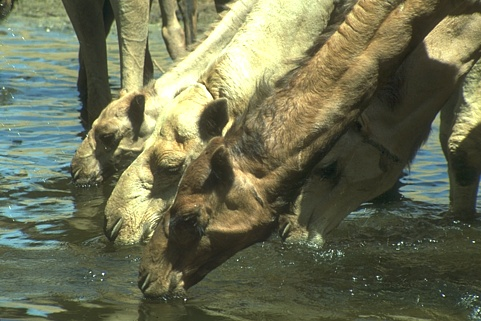
\includegraphics[width=\linewidth]{../../CBSD68/16077.png}\\[2pt]
    {\footnotesize Ground truth}
  \end{minipage}
  \\[8pt]
  \captionof{figure}{\texttt{16077.png} restored from $\sigma = 2$ blur. Read left to right, top to bottom.}
\end{center}

\clearpage
\begin{center}
  \begin{minipage}{0.48\linewidth}\centering
    
\includegraphics[width=\linewidth]{../blurred/sigma_2/19021.png}\\[2pt]
    {\footnotesize Blurry input --- 23.94\,dB / 0.6570}
  \end{minipage}%
  \hfill
  \begin{minipage}{0.48\linewidth}\centering
    
\includegraphics[width=\linewidth]{../deblurred-imgs/inverse/19021.png}\\[2pt]
    {\footnotesize Inverse filter --- 19.45\,dB / 0.3494}
  \end{minipage}
  \\[8pt]
  \begin{minipage}{0.48\linewidth}\centering
    
\includegraphics[width=\linewidth]{../deblurred-imgs/wiener/19021.png}\\[2pt]
    {\footnotesize Wiener filter --- 27.68\,dB / 0.8250}
  \end{minipage}%
  \hfill
  \begin{minipage}{0.48\linewidth}\centering
    
\includegraphics[width=\linewidth]{../deblurred-imgs/wiener-oracle/19021.png}\\[2pt]
    {\footnotesize Wiener filter (oracle) --- 27.88\,dB / 0.8203}
  \end{minipage}
  \\[8pt]
  \begin{minipage}{0.48\linewidth}\centering
    
\includegraphics[width=\linewidth]{../deblurred-imgs/cls-laplacian/19021.png}\\[2pt]
    {\footnotesize Constrained least squares --- 27.66\,dB / 0.8266}
  \end{minipage}%
  \hfill
  \begin{minipage}{0.48\linewidth}\centering
    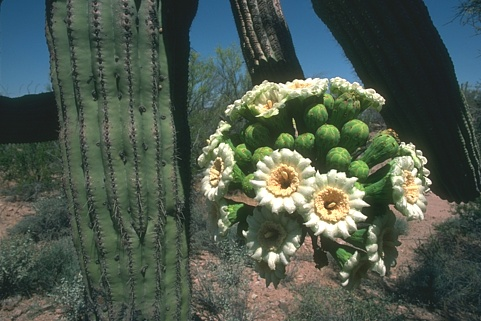
\includegraphics[width=\linewidth]{../../CBSD68/19021.png}\\[2pt]
    {\footnotesize Ground truth}
  \end{minipage}
  \\[8pt]
  \captionof{figure}{\texttt{19021.png} restored from $\sigma = 2$ blur. Read left to right, top to bottom.}
\end{center}

\clearpage
\begin{center}
  \begin{minipage}{0.48\linewidth}\centering
    
\includegraphics[width=\linewidth]{../blurred/sigma_2/24077.png}\\[2pt]
    {\footnotesize Blurry input --- 21.68\,dB / 0.7534}
  \end{minipage}%
  \hfill
  \begin{minipage}{0.48\linewidth}\centering
    
\includegraphics[width=\linewidth]{../deblurred-imgs/inverse/24077.png}\\[2pt]
    {\footnotesize Inverse filter --- 19.82\,dB / 0.4414}
  \end{minipage}
  \\[8pt]
  \begin{minipage}{0.48\linewidth}\centering
    
\includegraphics[width=\linewidth]{../deblurred-imgs/wiener/24077.png}\\[2pt]
    {\footnotesize Wiener filter --- 27.76\,dB / 0.8996}
  \end{minipage}%
  \hfill
  \begin{minipage}{0.48\linewidth}\centering
    
\includegraphics[width=\linewidth]{../deblurred-imgs/wiener-oracle/24077.png}\\[2pt]
    {\footnotesize Wiener filter (oracle) --- 28.21\,dB / 0.8835}
  \end{minipage}
  \\[8pt]
  \begin{minipage}{0.48\linewidth}\centering
    
\includegraphics[width=\linewidth]{../deblurred-imgs/cls-laplacian/24077.png}\\[2pt]
    {\footnotesize Constrained least squares --- 27.75\,dB / 0.9015}
  \end{minipage}%
  \hfill
  \begin{minipage}{0.48\linewidth}\centering
    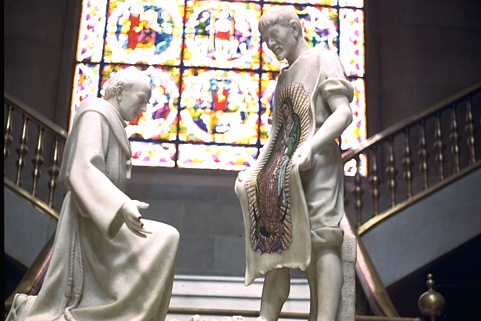
\includegraphics[width=\linewidth]{../../CBSD68/24077.png}\\[2pt]
    {\footnotesize Ground truth}
  \end{minipage}
  \\[8pt]
  \captionof{figure}{\texttt{24077.png} restored from $\sigma = 2$ blur. Read left to right, top to bottom.}
\end{center}


\end{document}
